%%%%%%%%%%%%%%%%%%%%%%%%%%
%%% author : Yamada. T %%%
%%% made for TH series %%%
%%%%%%%%%%%%%%%%%%%%%%%%%%

\documentclass[b5paper,10pt,fleqn] {ltjsarticle}

\usepackage[margin=10truemm]{geometry}

\usepackage{pict2e, graphicx}
\usepackage{tikz}
\usetikzlibrary{intersections,calc,arrows.meta}

\usepackage{amsmath, amssymb, amsthm}
\usepackage{ascmac}
\usepackage{comment}
\usepackage{empheq}
\usepackage[shortlabels,inline]{enumitem}
\usepackage{fancybox}
\usepackage{fancyhdr}
\usepackage{here}
\usepackage{lastpage}
\usepackage{listings, jvlisting}
\usepackage{fixdif}

\usepackage{stmaryrd}
\usepackage[listings]{tcolorbox}
%\usepackage{ascolorbox}
\usepackage{titlesec}
\usepackage{ulem}
\usepackage{url}
\usepackage{verbatim}
\usepackage{wrapfig}
\usepackage{xcolor}
\usepackage{luatexja-ruby}
\usepackage{varwidth}
\usepackage[version=3]{mhchem}
\usepackage{wrapfig}


\usepackage{physics2}
	\usephysicsmodule{ab}
	\usephysicsmodule{ab.braket}
	\usephysicsmodule{ab.legacy}
	%\usephysicsmodule{braket}
	\usephysicsmodule{diagmat}
	\usephysicsmodule{xmat}
	\usephysicsmodule{nabla.legacy}
	\usephysicsmodule{qtext.legacy}

\usepackage[ISO]{diffcoeff}
\difdef { f, s } { D }
{ op-symbol = \mathrm{D} }


\newcommand{\mctext}[1]{\mbox{\textcircled{\scriptsize{#1}}}}
\newcommand{\ctext}[1]{\textcircled{\scriptsize{#1}}}
\newcommand{\ds}{\displaystyle}
\newcommand{\comb}[2]{{}_{#1}\mathrm{C}_{#2}}
\newcommand{\hs}{\hspace}
\newcommand{\vs}{\vspace}
\newcommand{\emphvs}{\vspace{1em}\notag\\}
\newcommand{\ora}{\overrightarrow}
\newcommand{\ol}{\overline}
\newcommand{\oramr}[1]{\overrightarrow{\mathrm{#1}}}
\newcommand{\tri}{\triangle}
\newcommand{\mr}{\mathrm}
\newcommand{\mb}{\mathbb}
\newcommand{\mrvec}[1]{\overrightarrow{\mathrm{#1}}}
\newcommand{\itvec}{\overrightarrow}
\newcommand{\bs}{\boldsymbol}
\newcommand{\ra}{\rightarrow}
\newcommand{\Ra}{\Rightarrow}
\newcommand{\lra}{\longrightarrow}
\newcommand{\Lra}{\Longrightarrow}
\newcommand{\la}{\leftarrow}
\newcommand{\La}{\Leftarrow}
\newcommand{\lla}{\longleftarrow}
\newcommand{\Lla}{\Longleftarrow}
\newcommand{\lr}{\leftrightarrow}
\newcommand{\llr}{\longleftrightarrow}
\newcommand{\Llr}{\Longleftrightarrow}
\renewcommand{\deg}{{}^\circ}
\newcommand{\phbox}{\fbox{\phantom{1\hspace{2em}}}}
\newcommand{\boxnum}[1]{\fbox{\phantom{\hspace{1em}}({#1})\phantom{\hspace{1em}}}}
\newcommand{\boxkana}[1]{\fbox{\phantom{\hspace{1em}}{#1}\phantom{\hspace{1em}}}}
\newcommand{\boxkm}[2]{\fbox{\, {#1}\phantom{\hspace{0.2em}} \,  {#2}}}
\newcommand{\hzw}{\hspace{1\zw}}

\renewcommand{\baselinestretch}{1.25}
\parindent=1\zw

%入213

\begin{document}
\noindent\fbox{NewTH4-20} [横浜国立大]

\begin{wrapfigure}{r}{8cm}
  \centering
  \begin{minipage}{3.5cm}
    \centering
    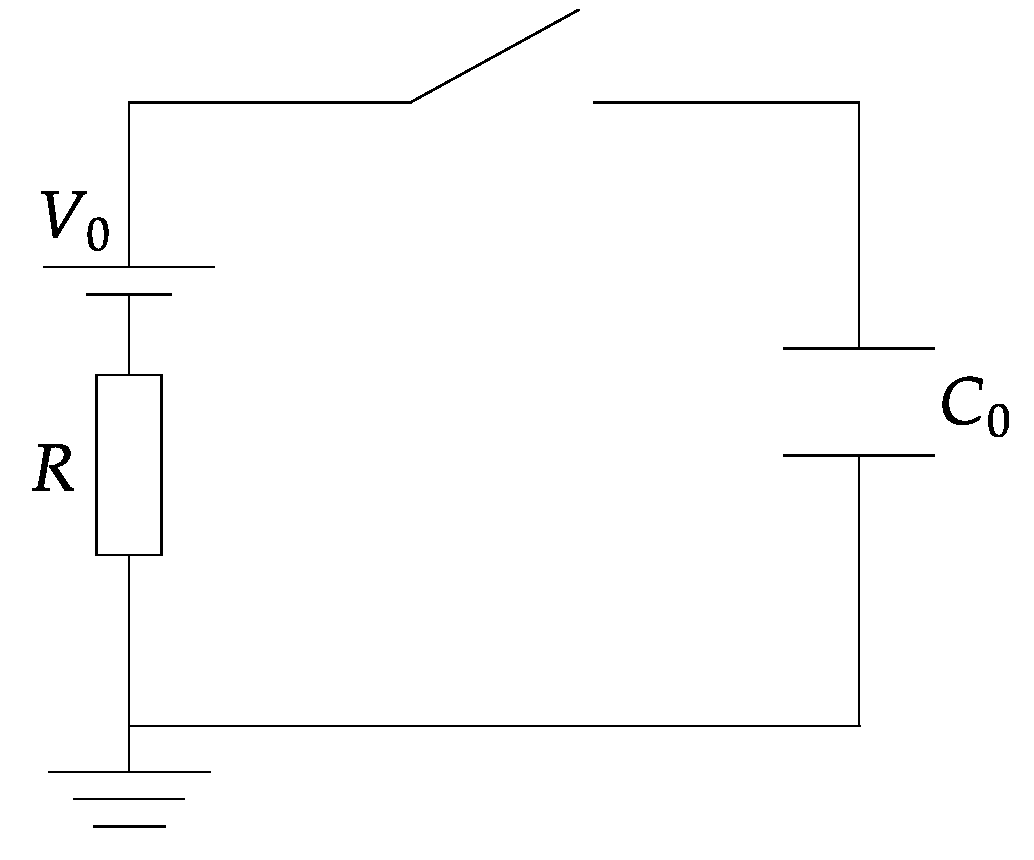
\includegraphics[width=3.5cm]{fig/fig_4_20_1.pdf}
    \caption{}
  \end{minipage}
  \hspace{1em}
  \begin{minipage}{3.8cm}
    \centering
    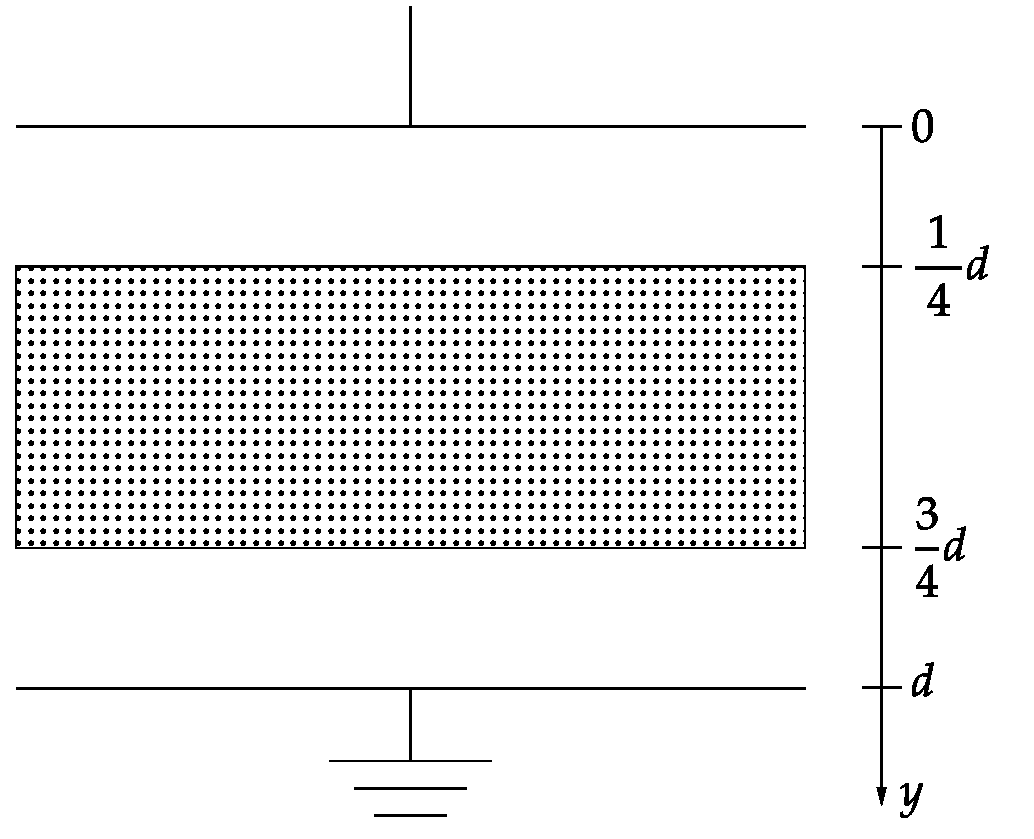
\includegraphics[width=3.5cm]{fig/fig_4_20_2.pdf}
    \caption{}
  \end{minipage}
\end{wrapfigure}
極板の面積$S$〔$\mr{m}^2$〕,間隔$d$〔$\mr{m}$〕の平行板コンデンサーがある.
図1のように,コンデンサーにはスイッチを通して起電力$V_0$〔$\mr{V}$〕の電池がつながれている.
ここで,抵抗$R$〔$\Omega$〕は電池の内部抵抗であり,導線の抵抗は無視する.
コンデンサーの負側の極板は接地されている.
スイッチを閉じてコンデンサーを充電し,十分に時間がたった後スイッチを開く.
このとき,コンデンサーに蓄えられた電荷を$Q_0$〔$\mr{C}$〕とする.
極板の端の影響は無視できるものとする.
以下の文章の空欄を埋めよ.
空欄\boxkana{オ}には適切な語を記入せよ.
空欄\boxkana{サ}と\boxkana{セ}には,問題文の最後にある選択肢\mctext{1}〜\mctext{3}から正しいものを選び記号で答えよ.
その他の空欄については,適切な数式を本文中の記号$Q_0$,$S$,$d$,$\varepsilon_0$,$\varepsilon_r$および数字を使って答えよ.また,(3)と(4)に従ってグラフを描け.

\begin{enumerate}[(1)]
  \item 極板間は真空であるとし,真空の誘電率を$\varepsilon_0$〔$\mr{F}/\mr{m}$〕とする.
    極板間の電気力線の本数はコンデンサーの電荷$Q_0$に比例し,極板間の電界の強さ$E$〔$\mr{V} / \mr{m}$〕は単位面積あたりの電気力線の本数に等しいから,電界の強さは,$E = \text{\boxkana{ア}} Q_0$である.
    したがって,充電電圧$V_0$とコンデンサーの電荷$Q_0$との関係は$Q_0 = \text{\boxkana{イ}}V_0$となり,この比例定数がコンデンサーの電気容量$C_0$〔$\mr{F}$〕を与える.
    ここで,電池がコンデンサーを充電するのに要した仕事$W$〔$\mr{J}$〕は$\text{\boxkana{ウ}}V_0$であり,コンデンサーに蓄えられた静電エネルギー$U_0$〔$\mr{J}$〕は$\text{\boxkana{エ}}V_0$である.その差は\boxkana{オ}として消費される.
  \item 極板間にはたらく力$F$〔$\mr{N}$〕を求めたい.極板間隔$d$における静電エネルギーは$U_0 = \text{\boxkana{カ}}d$と表される.極板をゆっくりと$\varDelta d$〔$\mr{m}$〕だけ引き離すときの静電エネルギーの変化分$\varDelta U$〔$\mr{J}$〕は外から加えた仕事$F \varDelta d$に等しい.
    これより,$F = \text{\boxkana{キ}}Q_0{}^2 = \text{\boxkana{ク}} Q_0 E$となることがわかる.
  \item スイッチを開いた状態で,図2のようにコンデンサーの中央に,極板と同じ大きさで厚みが$\dfrac{d}{2}$の電荷をもたない導体を挿入した.このときのコンデンサーの電気容量は導体挿入前の\boxkana{ケ}倍となる.
    図2に示すように,正側の極板上を座標の原点として負側の極板に向けて$y$軸をとるとき,$0 \leqq y \leqq d$における電位変化の様子を$V$--$y$グラフで描け.
    また,コンデンサーに蓄えられた静電エネルギーは導体挿入前の\boxkana{コ}倍となるから,導体は挿入時,\boxkana{サ}ことがわかる.
  \item (3)と同様に,スイッチを開いた状態で,コンデンサーの中央に,極板と同じ大きさで厚みが$\dfrac{d}{2}$,比誘電率が$\varepsilon_r\, (>1)$の帯電していない誘電体を挿入した.このときのコンデンサーの電気容量は,誘電体挿入前の\boxkana{シ}倍となる.$\varepsilon_r = 2$の場合について,$0 \leqq y \leqq d$における電位変化の様子を$V$--$y$グラフで描け.
    また,この場合にコンデンサーに蓄えられた静電エネルギーは誘電体挿入前の\boxkana{ス}倍となるから,誘電体挿入時,\boxkana{セ}ことがわかる.
    
    \begin{enumerate}[label=\mctext{\arabic*}]
      \item コンデンサーに引き込まれる力を受ける
      \item コンデンサーから押し出される力を受ける
      \item コンデンサーから力を受けない
    \end{enumerate}

\end{enumerate}
\end{document}
